\documentclass[uct_visualisation_thesis.tex]{subfiles}

\section{Instalacja}
\subsection{Wymagania sprzętowe}
W celu wykorzystania możliwości, które daje prezentowany system, należy uruchomić go na komputerze, który spełnia wymienione poniżej wymagania sprzętowe.

\begin{enumerate}
	\item Procesor: Intel Core i5-3470 3.2 GHz / AMD FX-8350 4 GHz.
	\item Pamięć RAM: 8 GB.
	\item Karta graficzna: Nvidia GTX 660 2GB / AMD HD 7870 2 GB.
	\item Miejsce na dysku twardym: 150 MB.
	\item System operacyjny: Windows 10 / Ubuntu 16.04.
\end{enumerate}

\subsection{Instrukcja instalacji Windows}
Aby zainstalować aplikację na dysku lokalnym, należy uruchomić plik instalacyjny \textit{UCTVisualisationSetup.exe}. Następnie ukaże się okno przeprowadzające użytkownika przez proces instalacji. Należy wybrać folder docelowy i kliknąć przycisk \textit{Install}. Po zakończeniu procesu można zamknąć okno instalacji, zaznaczając przedtem \textit{Run UCT Visualisation}, aby bezpośrednio po zamknięciu instalatora uruchomiła się aplikacja.\\

Zainstalowana aplikacja znajduje się w folderze wskazanym przez użytkownika podczas instalacji w katalogu \textit{UCT Visualisation}. Aby uruchomić aplikację należy w niego wejść i uruchomić plik \textit{UCT Visualisation.exe}.
Okno instalacji powinno przypominać to, ukazane na rysunku \ref{rys:instalacja}.

\begin{figure}[h!]
	\centering
	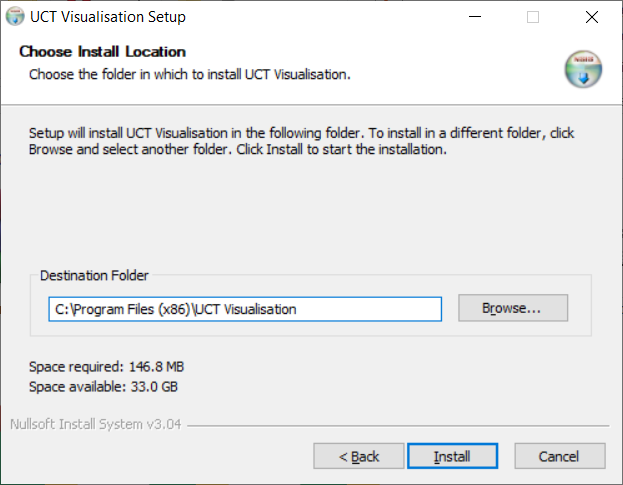
\includegraphics[width=0.7\textwidth]{instalacja}
	\caption{Okno instalacji programu - Windows}
	\label{rys:instalacja}
\end{figure}

\subsection{Instrukcja instalacji Linux}
W celu instalacji programu na lokalnym dysku, potrzebne jest uruchomienie pliku \textit{UCTVisualisationSetup.deb}, a następnie kliknięcie przycisku \textit{Install}, tak jak na rysunku \ref{rys:instalacja_linux}. 
Aplikacja o nazwie \textit{UCT Visualisation} znajduje się w katalogu o takiej samej nazwie i domyślnie zostaje zainstalowana pod ścieżką:
\begin{lstlisting}[style=mystylenonumbers]
/opt/"UCT Visualization"
\end{lstlisting}
zatem w celu uruchomienia aplikacji należy wpisać w systemowym terminalu następującą komendę:
\begin{lstlisting}[style=mystylenonumbers]
/opt/"UCT Visualization"/"UCT Visualization"
\end{lstlisting}
lub:
\begin{lstlisting}[style=mystylenonumbers]
cd /opt/"UCT Visualization"
./"UCT Visualization"
\end{lstlisting}

\begin{figure}[h!]
	\centering
	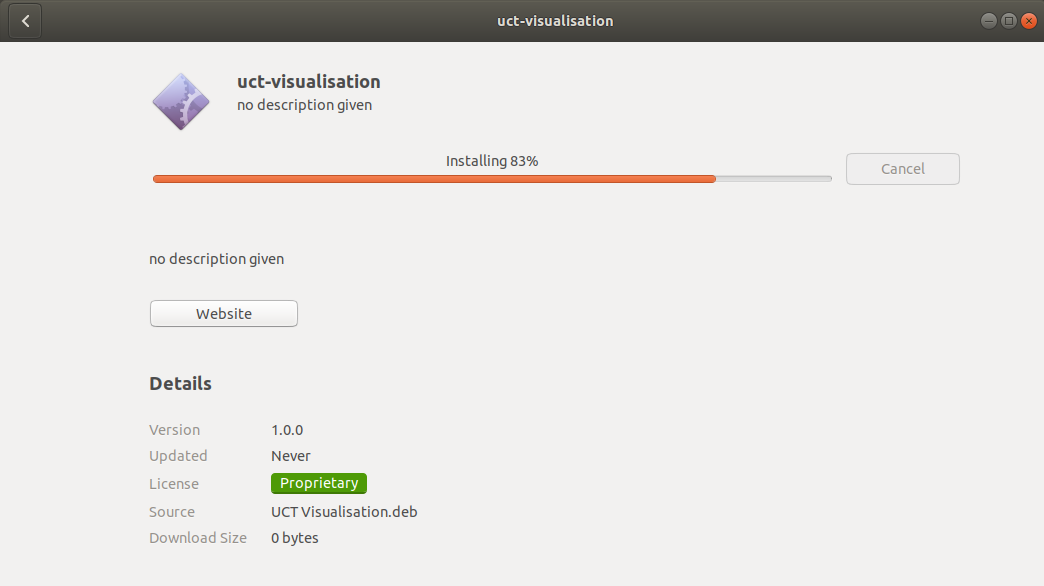
\includegraphics[width=0.9\textwidth]{ubuntu-installer}
	\caption{Okno instalacji programu - Ubuntu}
	\label{rys:instalacja_linux}
\end{figure}

\section{Mankala}
\subsection{Wstęp}
Mankala, jako jedna z przykładowych gier modułu \textit{Gry}, jest mniej popularną grą logiczną, więc postanowiono przedstawić instrukcję grania w nią.

Plansza mankali zawiera dwanaście mniejszych pól i dwa większe, nazywane domami. Każdy z graczy ma sześć mniejszych pól leżących przed nim i dom po jego prawej stronie. Na początku gry w każdym z pól znajdują się cztery kamienie. Celem obu graczy jest zebranie w domu jak największej liczby kamieni w ich domach. Gra kończy się, gdy wszystkie pola jednego z graczy są puste. Wtedy pozostałe kamienie przydzielane są drugiemu graczowi.

\begin{figure}[h!]
	\centering
	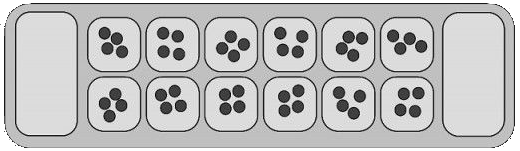
\includegraphics[width=0.6\textwidth]{mancala.png}
	\caption{Plansza mankali}
	\label{rys:mancala}
\end{figure}

\subsection{Ruch gracza}
Ruch gracza polega na wyjęciu wszystkich kamieni z wybranego własnego pola i rozdysponowaniu po jednym do kolejnych pól, omijając dom przeciwnika. Rozdysponowanie jest wykonywane w kierunku odwrotnym do ruchu wskazówek zegara. Ponadto, jeśli ostatni kamień wyląduje we własnym domu -- gracz musi wykonać kolejny ruch. Jeśli nie -- następuje ruch przeciwnika.

\subsection{Bicie}
Ostatnią zasadą mankali jest bicie. Bicie następuje, jeśli po wykonaniu ruchu, ostatni kamień wyląduje na pustym polu gracza. W takiej sytuacji gracz zabiera wszystkie kamienie z przyległego pola po drugiej stronie planszy. Jeżeli w sąsiednim polu nie ma kamieni, żaden kamień nie zostaje zbijany. Tak samo, ruch nie kończy się biciem, jeżeli ostatni kamień wyląduje na pustym polu przeciwnika.